I dette kapitel beskrives implementeringen af app'en, der omhandler tranformationen fra design til kode. Det vil beskrives, hvilken platform koden implementers gennem samt, hvilken designklasser der implementeres. Disse designklasser opdeles i implementering af grænseflader samt implementering af model og controller klasser. Databasen samt kommunikation med denne vil ligeledes indrages for således at give et indblik i, hvordan dette er implementeret. Ydermere vil de centrale elementer i app'en beskrives. Disse elementer omhandler tilpasning af træningsniveau samt resultater for brugeren. Overordnet vil beskrivelserne tage udgangspunkt i udpluk af den implementeret kode.

I \autoref{cha:design} er analyse- og designklasser samt funktionsnavne navngivet på dansk, hvorfor bogstaverne æ, ø og å forekommer. Disse symboler anvendes ikke under implementeringen.

\section{Implementeringsplatform}
Det er valgt at implementere app'en i Android Studio version 2.3.1 og programmere i Java, da dette er et objektorienteret programmeringssprog \citep{Brahma2015}. Android Studio er et officelt Integrated Development Environment (IDE) for udvikling af android app's \citep{android2017}, hvilket er passende for udviklingenen af dette projekts problemløsning. 

Strukturen i Android Studio opdeles i \textit{manifests}, \textit{res} samt \textit{java} mapper. \textit{Manifests} mappen indeholder en \textit{AndroidManifest.xml} fil, der er essentiel for, at app'en kan køre og indeholder aktiviter, der er implementeret. I denne fil er der derudover defineret tilladelser for den givne app. For udvikling af denne app har det været nødvendigt at tillade brug af internet samt GPS, for således at kunne tilgå databasen og beregne afstand i relation til konditionstræningen. 
\textit{Res} mappen indeholder ikke-kode ressourcer, der eksempelvis er de forskellige layouts.
Javaklasserne, der er oprettet i forbindelse med udviklingen af app'en er placeret i \textit{java} mappen.\citep{android2017}
 

\section{Implementering af grænseflader}
Til at implemteregrænseflader i systemet benyttes XML-filer, der håndteres i deres respektive controllere. I disse filer er det muligt at definere, hvilke type elemtenter, der skal indgå i layoutet. Dertil kan typen af layout defineres alt efter, hvordan layoutet skal opstilles. Layouts brugt i dette system er af type linear og relativ layouts.  

Elementer opstilles i layouts med type, størrelse samt orientering. Forekommer det, at elementerne skal benyttes i javakoden, defineres disse ligeledes med et id. Et eksempel af layoutkode fra log ind ses af \autoref{fig:logindlay}.

\begin{figure} [H]
\centering
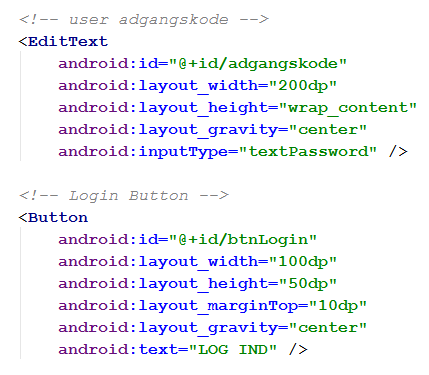
\includegraphics[width=0.6\textwidth]{figures/imple/logindlay}
\caption{Udklip af kode fra log ind layout. Udklippet viser et \textit{EditText}, hvori brugeren angiver adgangskode samt en button for log ind.}
\label{fig:logindlay}
\end{figure}

\noindent
Af dette udklip ses koden for tekstfeltet, hvori brugeren angiver adgangskode samt koden for layoutet af log ind-knappen. Feltet for adgangskoden er her af typen \textit{EditText}, der tillader, at brugeren kan angive tekst. Dette felt har ligeledes et id, der muliggøre at referere til feltet og hente den angivet adgangskode til validering af log ind. Knappen er opstillet af typen button, og har ligeledes et id, hvortil en listener er opstillet i javakoden. Dette er yderligere beskrevet i \autoref{sec:impmodelcon}.

\section{Implementering af model og controllerklasser} \label{sec:impmodelcon}
Model og controllerklasser er implementeret i \textit{Java Class} filer. Heri er klasser defineret med navn samt tilhørende antributter og metoder. Af \autoref{fig:javaclass} ses et eksempel på, hvordan en controller er implementeret. 

\begin{figure} [H]
\centering
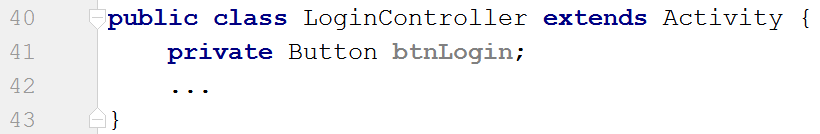
\includegraphics[width=0.6\textwidth]{figures/imple/javaclass}
\caption{Udpluk af javaklassen for LoginController. Punktumerne symboliserer den resterne kode, der ikke anses nødvendig for forklaring af opsætning af javaklasser.}
\label{fig:javaclass}
\end{figure}

Det fremgår af dette udklip, at klassen, \textit{LoginController}, er af typen public og nedarver \textit{activity}. Dette gør sig gældende for samtlige klasser implementeret. Denne klasse for \textit{LoginController} har attributten \textit{btnLogin}, der referer til log ind knappen på grænsefladen. Idet app'en skal reagerer, når brugeren trykker på btnLogin opsættes en listener på knappen, hvilket ses af \autoref{fig:list}.

\begin{figure} [H]
\centering
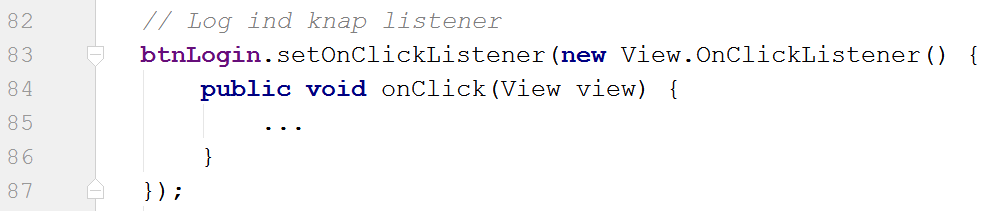
\includegraphics[width=0.6\textwidth]{figures/imple/list}
\caption{Udpluk af koden for listeneren opsat for log ind knappen. Punktumerne symboliserer den resterne kode, der ikke anses nødvendig for forklaring af opsætning af listener.}
\label{fig:list}
\end{figure}

Af dette udklip ses den opsatte listener, der har til formål at lytte på knappen. Indenfor listeneren er der opstillet kode, hvilket symboliseres ved punktumer, der køres idet der trykkes på knappen. Denne listener er ligeledes implementeret for samtlige knapper i controllerklasserne. Listeneren er implementeret i controllerklasserne, da det er disse filer, som håndterer input for de tilhørende layouts.

Modelklasserne er implementeret på samme vis som controllerklasserne, de har dog til formål at lagre data forinden det sendes til databasen. I disse klasser er der ligeledes opstilles attributter med tilhørende get og set metoder. 

